\begin{wrapfigure}[0]{r}[9pt]{0cm}
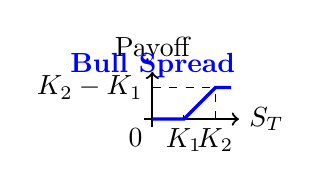
\begin{tikzpicture}[scale=1]
    % --- 定义坐标和参数 ---
    \def\Kone{0.4}       % 行权价 K1
    \def\Ktwo{0.8}       % 行权价 K2 (K2 > K1)
    \def\maxST{1}      % S_T 的最大显示范围
    \def\maxPayoff{\Ktwo - \Kone} % 最大收益 (K2 - K1)

    % --- 绘制坐标轴 ---
    % X 轴 (S_T)
    \draw[->, thick] (-0.1, 0) -- (\maxST + 0.1, 0) node[right] {$S_T$};
    % Y 轴 (Payoff)
    \draw[->, thick] (0, -0.1) -- (0, \maxPayoff + 0.2) node[above] {Payoff};

    % --- 绘制辅助线和标签 ---
    % 标记原点
    \node[below left] at (0, 0) {0};

    % 在 X 轴上标记 K1
    \draw (\Kone, 0) node[below] {$K_1$} -- (\Kone, 0.05); % 短刻度线

    % 在 X 轴上标记 K2，并向上画虚线
    \draw (\Ktwo, 0) node[below] {$K_2$} -- (\Ktwo, 0.05); % 短刻度线
    \draw[dashed, thin] (\Ktwo, 0) -- (\Ktwo, \maxPayoff);

    % 在 Y 轴上标记最大收益 K2 - K1，并向右画虚线
    \draw (0, \maxPayoff) node[left] {$K_2 - K_1$} -- (0.05, \maxPayoff); % 短刻度线
    \draw[dashed, thin] (0, \maxPayoff) -- (\Ktwo, \maxPayoff);


    % --- 绘制牛市价差收益曲线 (蓝色粗线) ---
    % 路径: (0,0) -> (K1, 0) -> (K2, K2-K1) -> (maxST, K2-K1)
    \draw[blue, very thick] (0, 0) -- (\Kone, 0) -- (\Ktwo, \maxPayoff) -- (\maxST, \maxPayoff);

    % --- 添加标题标签 ---
    % 将标题放在图像的右上方
    \node[blue, anchor=south east, font=\bfseries,xshift= 5pt] at (\maxST, \maxPayoff) {Bull Spread};

\end{tikzpicture}
\end{wrapfigure}